\documentclass[aspectratio=169, 14pt]{beamer}
\input{preamble}

\title{Large Language Models}
\subtitle{A Physicist's Perspective}

\begin{document}

% =====================================================================
% TITLE
% =====================================================================

\begin{frame}[plain]
  \titlepage
\end{frame}

% =====================================================================
% SECTION 0: WHY THIS TALK?
% =====================================================================

\sectiondivider{Why this talk?}

% --- GPT-5.2 headline ---
\begin{frame}[plain]
  \vfill
  \centering
  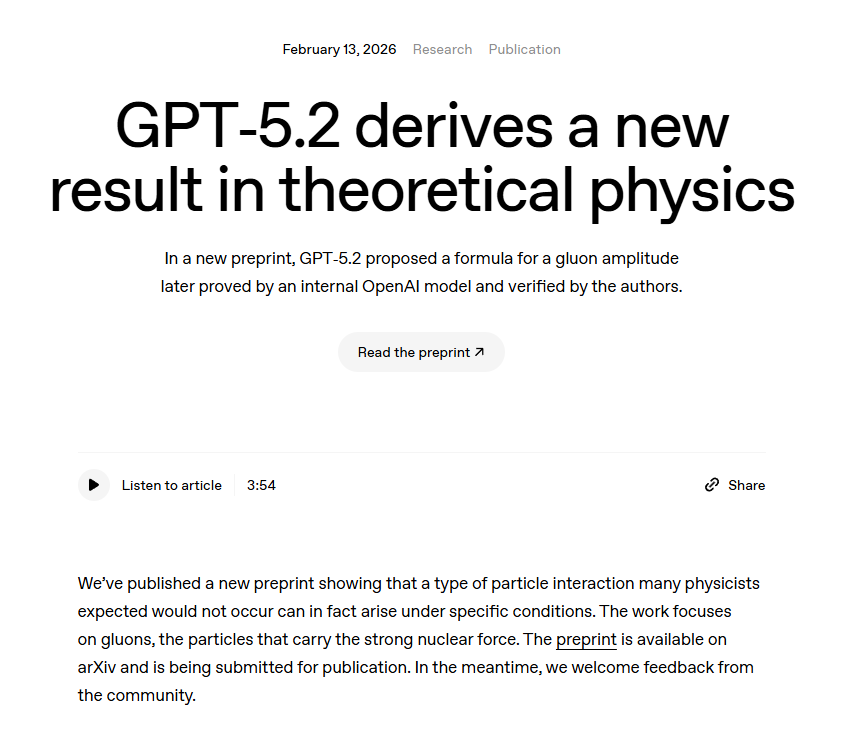
\includegraphics[width=0.85\textwidth]{assets/gpt52pr.PNG}

  \vskip1em
  {\small\color{tjo@black!60}%
    arXiv:2602.12176 \quad---\quad
    IAS, Harvard, Cambridge, Vanderbilt, OpenAI \quad---\quad
    February 2026}
  \vfill
\end{frame}

% --- Timeline ---
\begin{frame}{Three moments}
  \vfill
  \centering
  \begin{tikzpicture}[
    event/.style={
      tjo box,
      minimum width=3.2cm,
      minimum height=1.8cm,
      font=\normalsize,
      align=center,
    },
  ]
    % Timeline axis
    \draw[tjo@black!20, line width=2pt] (-5.5,0) -- (5.5,0);

    \node[event, fill=tjo@lightgrey] (gpt) at (-4,0) {%
      {\bfseries\color{tjo@darkteal} Nov 2022}\\[3pt]
      ChatGPT\\launches
    };

    \node[event, fill=tjo@lightgrey] (cc) at (0,0) {%
      {\bfseries\color{tjo@darkteal} Q1 2025}\\[3pt]
      Claude Code,\\Cursor, Copilot
    };

    \node[event, fill=tjo@lightgrey] (good) at (4,0) {%
      {\bfseries\color{tjo@darkteal} Q4 2025}\\[3pt]
      Opus 4.5, GPT-5.2\\cross a threshold
    };
  \end{tikzpicture}
  \vfill
\end{frame}

% --- Audience poll ---
\begin{frame}{Quick survey: experience}
  \vfill
  \centering
  {\fontsize{20}{26}\selectfont
    \begin{tabular}{l}
      \color{tjo@cyan}$\bullet$\quad used ChatGPT, Claude, or Gemini \\[0.8em]
      \color{tjo@cyan}$\bullet$\quad used an LLM in your IDE to write code \\[0.8em]
      \color{tjo@cyan}$\bullet$\quad used a coding agent \\
    \end{tabular}
  }
  \vfill
\end{frame}

% --- Personal confession ---
\statementslide{If you experimented with chat in Q1 2025,\\[0.5em]
  you probably dismissed LLMs\\[0.8em]
  {\fontsize{20}{26}\selectfont\mdseries I did}}

% --- Skeptic ---
\statementslide{I was a skeptic\\[0.8em]
  {\fontsize{20}{26}\selectfont\mdseries
    I am still annoyed at the models of Q1 2025}}

% --- The problem (quote) ---
\statementslide{\textit{``LLMs are \textbf{incredibly capable}}\\[0.5em]
  \textit{but \textbf{maximally untrustworthy}''}}

% --- The evidence ---
\begin{frame}{The evidence}
  \vfill
  \centering
  Seductively correct equations that are nonsense

  \vskip1.5em
  Push back on a valid proof and the LLM finds a ``bug'' that isn't there

  \vskip1.5em
  They lie, cheat, steal, and flatter

  \vskip2em
  {\color{tjo@darkteal}\bfseries All terrible qualities for reproducible science}
  \vfill
\end{frame}

% --- Mental model ---
\statementslide{A good mental model of an LLM:\\[0.8em]
  a slightly deranged,\\[0.3em]
  hypermotivated MSc student}

% --- The gap ---
\begin{frame}[plain,c]
  \centering
  {\fontsize{22}{30}\selectfont\color{tjo@darkteal}
    The gap between\\[0.6em]
    {\bfseries ``I tried ChatGPT and it hallucinated''}\\[0.6em]
    and\\[0.6em]
    {\bfseries ``this is a powerful force multiplier''}\\[0.8em]
  }
  {\fontsize{20}{26}\selectfont\color{tjo@darkteal}
    is not closed by better models\\[0.5em]
    It is closed by \textbf{technique} and \textbf{domain expertise}
  }
\end{frame}

% --- Three requirements ---
\begin{frame}{What it takes}
  \vfill
  \centering
  {\fontsize{20}{28}\selectfont
    \begin{tabular}{r@{\hspace{0.8em}}l}
      \color{tjo@darkteal}\bfseries 1 &
        Deliberate practice --- a different workflow \\[1em]
      \color{tjo@darkteal}\bfseries 2 &
        A subscription --- free chat is not enough \\[1em]
      \color{tjo@darkteal}\bfseries 3 &
        A coding agent --- Claude Code, Cline, \ldots \\
    \end{tabular}
  }
  \vfill
\end{frame}

% --- Project showcase ---
\begin{frame}{With the correct workflow}
  \vfill
  \centering
  \renewcommand{\arraystretch}{1.4}
  {\fontsize{14}{19}\selectfont
  \begin{tabular}{l@{\hspace{1.2em}}l@{\hspace{1.2em}}l}
    \textbf{\color{tjo@darkteal}vibefeld}
      & Go, 112k lines
      & adversarial proof verification \\
    \textbf{\color{tjo@darkteal}Lyr.jl}
      & Julia
      & volume renderer, GR ray tracing \\
    \textbf{\color{tjo@darkteal}af-tests}
      & Lean\,4, 0 sorries
      & formal proofs in operator algebras \\
    \textbf{\color{tjo@darkteal}convexfeld}
      & C, 37k lines
      & LP solver from scratch \\
    \textbf{\color{tjo@darkteal}Nano MIPS}
      & Verilog
      & pipelined CPU on \$10 FPGA \\
  \end{tabular}
  }

  \vskip1.5em
  {\color{tjo@darkteal}\bfseries
    All with basic tooling --- no extra subscriptions}
  \vfill
\end{frame}

% --- Formalization ---
\statementslide{Auto formalization is real\\[0.8em]
  Writing new science is now possible}

% --- Accelerating research ---
\statementslide{Accelerating research is possible\\[0.8em]
  {\fontsize{20}{26}\selectfont\mdseries
    With correct tooling and expert guidance\\[0.3em]
    The human provides the ground truth}}

% --- Transition ---
\statementslide{LLMs can be understood\\[0.8em]
  {\fontsize{20}{26}\selectfont\mdseries
    Let me rebuild the stack from first principles}}

% =====================================================================
% SECTION 1: WHAT IS AN LLM?
% =====================================================================

\sectiondivider{What is an LLM?}

% --- From outside, looking in ---
\begin{frame}[fragile]{From outside, looking in}
  \vfill
  \centering
\begin{codeblock}
f : String -> String
\end{codeblock}
  \vskip1.5em
  From outside the API boundary, this is the entire observable behaviour

  \medskip
  No hidden state is carried between calls
  \vfill
\end{frame}

% --- Stateless ---
\begin{frame}{Stateless}
  \vfill
  \centering
  \begin{tikzpicture}
    \node[tjo box fill] (c1) {Call 1};
    \draw[tjo arrow] ([xshift=-2.5cm]c1.west) -- (c1.west)
      node[tjo label] {input};
    \draw[tjo arrow] (c1.east) -- ([xshift=2.5cm]c1.east)
      node[tjo label] {output};

    \node[tjo box fill, right=5cm of c1] (c2) {Call 2};
    \draw[tjo arrow] ([xshift=-2.5cm]c2.west) -- (c2.west)
      node[tjo label] {input};
    \draw[tjo arrow] (c2.east) -- ([xshift=2.5cm]c2.east)
      node[tjo label] {output};

    \draw[dashed, color=tjo@black!25, line width=1pt]
      ([xshift=1.8cm]c1.east) -- ([xshift=-1.8cm]c2.west)
      node[midway, font=\huge, text=red!70!black] {$\times$};
  \end{tikzpicture}

  \vskip1.5em
  Each evaluation is independent --- no memory between calls
  \vfill
\end{frame}

% --- Nondeterministic ---
\begin{frame}{Nondeterministic}
  \vfill
  \centering
  \begin{tikzpicture}
    \node[tjo box fill, minimum width=4cm] (input) {\texttt{"What is spin?"}};

    \node[tjo box, right=5cm of input, yshift=1.8cm]  (o1) {\texttt{"Spin is\ldots"}};
    \node[tjo box, right=5cm of input]                 (o2) {\texttt{"Angular\ldots"}};
    \node[tjo box, right=5cm of input, yshift=-1.8cm] (o3) {\texttt{"In QM\ldots"}};

    \draw[tjo arrow] (input.east) -- (o1.west);
    \draw[tjo arrow] (input.east) -- (o2.west);
    \draw[tjo arrow] (input.east) -- (o3.west);
  \end{tikzpicture}

  \vskip1em
  Same input, different outputs ---
  the model samples from $\Prob(\text{next token} \given \text{context})$
  \vfill
\end{frame}

% --- Probability distribution (NEW) ---
\statementslide{An LLM outputs a probability distribution\\[0.5em]
  over tokens\\[0.8em]
  Then it samples one}

% --- Temperature (formula) ---
\begin{frame}{Temperature}
  \vfill
  \[
    P(\text{token}_i) \;=\; \frac{\exp(\ell_i / T)}{\displaystyle\sum_j \exp(\ell_j / T)}
  \]

  \vskip1.5em
  \centering
  {\color{tjo@darkteal}\bfseries Direct analogy to the Boltzmann distribution}
  \vfill
\end{frame}

% --- Temperature limits ---
\begin{frame}{Temperature limits}
  \vfill
  \centering
  {\fontsize{24}{32}\selectfont
    $T \to 0$\;: deterministic \quad (ground state)
  }

  \vskip2em
  {\fontsize{24}{32}\selectfont
    $T \to \infty$\;: uniform \quad (infinite temperature)
  }
  \vfill
\end{frame}

% --- Tokens ---
\begin{frame}[fragile]{Tokens}
  \vfill
  Not characters. Not words.

  \medskip
  Subword chunks from a fixed vocabulary $V$ of ${\sim}100\text{k}$ entries.

  \vskip1.5em
\begin{codeblock}
'theoretical physics'  ->  ['theor', 'etical', ' physics']
\end{codeblock}

  \vskip1em
  {\small\color{tjo@black!60}
    More precisely: $f : \text{Token}^* \to \text{Token}^*$}
  \vfill
\end{frame}

% --- Inference ---
\statementslide{An LLM call =\\[0.5em]
  one forward pass through a frozen neural network\\[0.8em]
  No learning --- no state mutation}

% --- Closing statement ---
\begin{frame}[plain,c]
  \centering
  {\fontsize{20}{28}\selectfont\color{tjo@darkteal}
  An LLM is a stateless, nondeterministic function

  \vskip0.8em
  \[ f : \text{String} \to \text{String} \]

  \vskip0.8em
  that samples from $\Prob(\text{next\_token} \given \text{context})$

  \medskip
  via a single forward pass through a frozen neural network
  }
\end{frame}

% =====================================================================
% SECTION 2: THE ILLUSION OF CHAT
% =====================================================================

\sectiondivider{The illusion of chat}

% --- A single API call ---
\begin{frame}{You interact with an LLM via a single API call}
  \vfill
  \centering
  \begin{tikzpicture}
    \node[tjo box fill, minimum width=4cm] (client) {\textbf{Client}};
    \node[tjo box fill, minimum width=4cm, right=7cm of client] (api) {\textbf{API}};

    \draw[tjo arrow] ([yshift=0.5cm]client.east) -- ([yshift=0.5cm]api.west)
      node[midway, above, font=\normalsize] {prompt (string)};

    \draw[tjo arrow] ([yshift=-0.5cm]api.west) -- ([yshift=-0.5cm]client.east)
      node[midway, below, font=\normalsize] {completion (string)};
  \end{tikzpicture}

  \vskip1.5em
  {\large One string in --- one string out --- that is the entire interaction}
  \vfill
\end{frame}

% --- The cURL reality ---
\begin{frame}[fragile]{The cURL reality}
  \vfill
\begin{codeblock}
curl api.anthropic.com/v1/messages \
  -H "x-api-key: $KEY" \
  -H "content-type: application/json" \
  -d '{"model":"claude-sonnet-4-6-20250627",
       "messages":[{"role":"user",
         "content":"What is a quark?"}]}'
\end{codeblock}
  \vfill
\end{frame}

% --- The HTTP reality ---
\begin{frame}[fragile]{The HTTP reality}
  \vfill
\begin{codeblock}
POST /v1/messages
{
  "model": "claude-sonnet-4-6-20250627",
  "messages": [
    {"role": "user",
     "content": "What is a quark?"}
  ]
}
\end{codeblock}
  \vfill
\end{frame}

% --- How chat works ---
\begin{frame}[fragile]{How chat works}
  \vfill
\begin{codeblock}
Turn 1:  [user_1]
Turn 2:  [user_1, asst_1, user_2]
Turn 3:  [user_1, asst_1, user_2, asst_2, user_3]
\end{codeblock}

  \vskip1.5em
  The client re-sends the \textbf{entire} history every time
  \vfill
\end{frame}

% --- No memory ---
\statementslide{The LLM has no memory\\[0.8em]
  The client maintains the illusion}

% --- The context window (bar chart) ---
\begin{frame}{The context window}
  \vfill
  \centering
  \begin{tikzpicture}
    \fill[tjo@lightgrey] (0,0) rectangle (12,1.2);
    \fill[tjo@darkteal!30] (0,0) rectangle (2,1.2);
    \node[font=\small, text=tjo@darkteal, align=center] at (1,0.6) {system\\ prompt};
    \fill[tjo@cyan!20] (2,0) rectangle (9.5,1.2);
    \node[font=\small, align=center] at (5.75,0.6) {conversation history};
    \fill[tjo@cyan!40] (9.5,0) rectangle (12,1.2);
    \node[font=\small, align=center] at (10.75,0.6) {latest\\ message};
    \draw[tjo@darkteal, line width=1pt] (0,0) rectangle (12,1.2);
    \draw[decorate, decoration={brace, amplitude=8pt, mirror},
          tjo@darkteal, line width=1pt]
      (0,-0.3) -- (12,-0.3)
      node[midway, below=10pt, font=\normalsize] {context window (tokens)};
  \end{tikzpicture}

  \vskip1.5em
  When the conversation exceeds it, something must be dropped

  \vskip1em
  {\color{tjo@darkteal}\bfseries
    8k tokens {\mdseries(free chat)} \qquad
    128k--200k tokens {\mdseries(frontier models)}}
  \vfill
\end{frame}

% --- Context rot ---
\begin{frame}{Context rot}
  \vfill
  \centering
  As the context fills, older information gets buried

  \vskip1.5em
  The model's effective attention degrades

  \vskip1.5em
  Your constraints, instructions, and earlier results silently disappear

  \vskip2em
  {\color{tjo@darkteal}\bfseries
    This is why chat interfaces silently ruin your results}
  \vfill
\end{frame}

% --- The system prompt ---
\begin{frame}{The system prompt}
  \vfill
  A hidden preamble prepended to every call

  \vskip1em
  It shapes behaviour, persona, and constraints

  \vskip1.5em
  {\color{tjo@darkteal}\bfseries It is just more text}

  \vskip1.5em
  {\small\color{tjo@black!60}
    Anthropic's system prompt has been published --- it is just text\\
    \url{https://docs.anthropic.com/en/release-notes/system-prompts}}
  \vfill
\end{frame}

% --- Summary ---
\statementslide{Chat is a loop\\[0.8em]
  Memory is an illusion\\[0.3em] maintained by the client}

% =====================================================================
% SECTION 3: FROM FUNCTION TO AGENT
% =====================================================================

\sectiondivider{From function to agent}

% --- Two ways in ---
\begin{frame}{Two ways in}
  \vfill
  \centering
  \begin{tikzpicture}[node distance=4cm]
    \node[tjo box fill, minimum width=4.5cm, minimum height=2cm] (web)
      {\textbf{Web interface}\\[4pt]{\normalsize ChatGPT, Claude.ai}\\[2pt]
       {\small\color{tjo@black!60} chat UI hides the API}};
    \node[tjo box fill, minimum width=4.5cm, minimum height=2cm, right=3cm of web] (term)
      {\textbf{Terminal}\\[4pt]{\normalsize cURL, Python}\\[2pt]
       {\small\color{tjo@black!60} direct API access}};

    \draw[tjo arrow, <->] (web.east) -- (term.west)
      node[midway, above, font=\normalsize] {same API underneath};
  \end{tikzpicture}
  \vfill
\end{frame}

% --- The agent loop (code) ---
\begin{frame}[fragile]{The agent loop}
  \vfill
\begin{codeblock}
while not done:
    response = llm(system_prompt + history)
    tool_calls = parse(response)
    results = execute(tool_calls)
    history += [response, results]
\end{codeblock}

  \vskip1.5em
  {\color{tjo@darkteal}\bfseries
    This is the complete architecture of every coding agent}
  \vfill
\end{frame}

% --- The agent loop (diagram) ---
\begin{frame}{The agent loop}
  \vfill
  \centering
  \begin{tikzpicture}[node distance=1.6cm, every node/.style={align=center}]
    \node[tjo box, fill=tjo@darkteal, text=white, minimum width=4cm,
          minimum height=1cm, font=\normalsize]
      (sys) {System prompt + History};

    \node[tjo box fill, below=1.2cm of sys, minimum width=4cm,
          minimum height=1cm, font=\normalsize]
      (llm) {\textbf{LLM}\; {\small\code{f(s) $\to$ s}}};

    \node[tjo box, right=3cm of llm, minimum height=1cm, font=\normalsize]
      (parse) {Parse tool calls};

    \node[tjo box, below=1.2cm of parse, minimum height=1cm, font=\normalsize]
      (exec) {Execute tools};

    \draw[tjo arrow] (sys) -- (llm);
    \draw[tjo arrow] (llm) -- (parse)
      node[midway, above, font=\small] {response};
    \draw[tjo arrow] (parse) -- (exec)
      node[midway, right, font=\small] {call};

    % Results arrow: loop back around into LLM
    \draw[tjo arrow] (exec.south) -- ++(0,-0.6) -| ([xshift=-0.5cm]llm.south)
      node[near start, below, font=\small] {results};

    % Feedback to history
    \draw[tjo arrow, dashed, color=tjo@cyan]
      ([xshift=0.5cm]llm.north) -- ([xshift=0.5cm]sys.south)
      node[midway, right, font=\small, text=tjo@cyan] {append};
  \end{tikzpicture}
  \vfill
\end{frame}

% --- Tools ---
\begin{frame}{Tools}
  \vfill
  \centering
  You describe tools in the system prompt

  \vskip1.5em
  The LLM generates structured text requesting a tool call

  \vskip1.5em
  Your scaffolding parses and executes it
  \vfill
\end{frame}

% --- The key insight ---
\statementslide{The LLM never executes anything}

% --- Two tools ---
\begin{frame}[fragile]{Two tools}
  \vfill
  \centering
\begin{codeblock}
read_file(path)           -> contents
write_file(path, content) -> ok
\end{codeblock}

  \vskip1.5em
  {\color{tjo@darkteal}\bfseries That is enough to do useful work}
  \vfill
\end{frame}

% --- Production equivalence ---
\statementslide{Claude Code, Cursor, Copilot:\\[0.8em]
  the same loop, more tools,\\[0.3em] better prompts}

% --- Live demo ---
\statementslide{{\fontsize{36}{44}\selectfont LIVE DEMO}\\[1em]
  {\fontsize{20}{26}\selectfont\mdseries Watch the agent work}}

% =====================================================================
% SECTION 4: BEYOND THE LOOP
% =====================================================================

\sectiondivider{Beyond the loop}

% --- The real workflow ---
\begin{frame}{The real workflow}
  \vfill
  \centering
  You do not sit and watch the agent type

  \vskip1.5em
  You launch it, walk away, and check the result

  \vskip2em
  {\color{tjo@darkteal}\bfseries A bash loop is the simplest orchestrator}
  \vfill
\end{frame}

% --- Bash polling loop ---
\begin{frame}[fragile]{Bash polling loop}
  \vfill
\begin{codeblock}
while true; do
    claude --prompt "Fix the failing tests" \
           --output result.json
    if tests_pass result.json; then
        break
    fi
    sleep 10
done
\end{codeblock}

  \vskip1em
  {\color{tjo@darkteal}\bfseries Infrastructure = a \code{while} loop in bash}
  \vfill
\end{frame}

% --- Multi-agent orchestration ---
\begin{frame}{Multi-agent orchestration}
  \vfill
  \centering
  \begin{tikzpicture}[node distance=2cm, every node/.style={align=center}]
    \node[tjo box, fill=tjo@darkteal, text=white,
          minimum width=5cm, minimum height=1cm, font=\normalsize]
      (sup) {\textbf{Supervisor}\\{\small orchestrates the pipeline}};

    \node[tjo box fill, below left=1.5cm and 1cm of sup,
          minimum width=3.5cm, font=\normalsize]
      (a1) {\textbf{Agent 1}\\{\small writes code}};
    \node[tjo box fill, below=1.5cm of sup,
          minimum width=3.5cm, font=\normalsize]
      (a2) {\textbf{Agent 2}\\{\small reviews code}};
    \node[tjo box fill, below right=1.5cm and 1cm of sup,
          minimum width=3.5cm, font=\normalsize]
      (a3) {\textbf{Agent 3}\\{\small runs tests}};

    \draw[tjo arrow] (sup) -- (a1);
    \draw[tjo arrow] (sup) -- (a2);
    \draw[tjo arrow] (sup) -- (a3);

    \draw[tjo arrow, dashed, color=tjo@cyan] (a1.east) -- (a2.west);
    \draw[tjo arrow, dashed, color=tjo@cyan] (a2.east) -- (a3.west);
  \end{tikzpicture}

  \vskip1em
  One agent writes --- another reviews --- a third tests
  \vfill
\end{frame}

% --- The natural endpoint ---
\statementslide{Single function $\to$ agent $\to$ multi-agent\\[0.8em]
  {\fontsize{20}{26}\selectfont\mdseries The natural endpoint of the stack}}

% --- Be skeptical ---
\begin{frame}{Be skeptical}
  \vfill
  \centering
  Getting reliable research output requires\\[0.5em]
  understanding the limitations

  \vskip1.5em
  Every layer we built today has failure modes

  \vskip1.5em
  Context rot, hallucination, tool misuse, prompt fragility

  \vskip2em
  {\color{tjo@darkteal}\bfseries
    The human in the loop is not optional}
  \vfill
\end{frame}

% =====================================================================
% SECTION 5: LIVE CODING
% =====================================================================

\sectiondivider{Live coding}

\statementslide{{\fontsize{30}{38}\selectfont Let's try something}\\[1em]
  {\fontsize{20}{26}\selectfont\mdseries No promises}}

\end{document}
